% !Mode:: "TeX:UTF-8"
\chapter{实验设计与结果分析}
\label{cha:experiment}

本章将通过系统的实验验证基于Transformer的点云补全算法的有效性和优越性。实验设计涵盖对比实验和消融实验两个层面。对比实验旨在将本算法与当前主流的补全方法在相同的数据集和评价指标下进行公平比较，验证算法的整体性能优势。消融实验则通过逐项移除或替换算法中的关键组件，分析各个优化措施对最终补全质量的独立贡献，从而验证损失函数优化策略的合理性。

\section{实验环境与数据集}

\subsection{开发环境}

本算法的实验在一台配备NVIDIA RTX 5090 GPU（32GB显存）的工作站上完成。该显卡具备强大的并行计算能力和充足的显存容量，为大批量训练和高精度损失函数的计算提供了硬件保障。操作系统为Ubuntu22.04LTS，深度学习框架基于PyTorch实现。

训练过程中启用了自动混合精度（Automatic Mixed Precision, AMP）技术，通过动态选择FP16和FP32精度，在保持数值稳定性的同时显著降低了显存占用和计算时间。优化器选用AdamW，初始学习率设置为$1 \times 10^{-4}$，权重衰减系数为$5 \times 10^{-4}$。学习率调度采用LambdaLR策略，每21个epoch以0.9的衰减率递减，最低学习率限制为初始学习率的2\%。Batch Momentum和Batch Normalization的衰减策略与学习率调度保持一致，确保训练过程的稳定性。

% 模型的超参数配置如下：编码器采用6层几何感知Transformer模块，嵌入维度为384，注意力头数为6，K近邻数量为8，分组数为2，MLP扩展比率为2。解码器采用8层自注意力与交叉注意力交替的Transformer结构，配置与编码器保持一致。粗粒度点云数量设置为512，细粒度点云数量设置为8192。训练总epoch数为600，Batch Size大小为64。

% 在损失函数方面，EMD计算的迭代次数设置为2000次，在精度和计算效率之间取得平衡。DCD损失的温度参数$\gamma$设置为1000，排斥损失的半径阈值$r$设置为0.07，Gaussian核带宽参数$h$设置为0.03，锚点采样数量设置为2048，K近邻数量设置为5。这些参数的取值依据在后续章节中将进行详细分析。

% 实验所依赖软件环境包括PyTorch深度学习框架、CUDA并行计算平台以及一系列辅助库。数据处理方面使用NumPy进行数值计算，Open3D用于点云可视化和几何操作，OpenCV用于图像处理相关任务。训练过程的监控通过TensorBoardX实现，实时记录损失曲线和各项评价指标的变化趋势。配置文件管理采用YAML格式，结合EasyDict库实现配置参数的便捷访问。

\subsection{点云补全数据集}

本算法的实验评估采用ShapeNet-34数据集进行。该数据集基于ShapeNetCore三维形状数据库，选取了34个常见类别，涵盖飞机、汽车、椅子、桌子等具有代表性的人工物体。每个三维模型被预处理为包含8192个点的点云表示，训练集和测试集遵循标准的实验协议划分。点云数据在输入网络之前经过归一化处理，将所有点平移至以原点为中心并缩放至单位球范围内，消除了不同模型在尺度和位置上的差异。本文中ShapeNet-34数据集仅在训练中使用，用于控制变量，与其他主流算法进行对比实验，量化反映模型性能。

为进一步提升评估的挑战性和现实贴合度，PoinTr项目提出了Projected-ShapeNet数据集。由于ShapeNet-34作为纯合成数据集，难以验证算法在实际应用场景中的性能；当前领域内主要使用KITTI数据集（纯真实采集数据集）验证算法的实际落地性能，但使用KITTI数据集进行训练存在硬件需求门槛高的问题。由于本文实验环境的硬件条件有限，故使用Projected-ShapeNet作为轻量化的仿真实采集数据集，应用于可视化展示模型实际落地能力。该数据集采用投影渲染的方式生成残缺点云：从多个随机视角对完整三维模型进行深度图渲染，再将深度图反投影为点云。与随机裁剪相比，投影渲染产生的残缺模式更加接近真实观测设备的特性，例如遮挡导致的结构性缺失和视角限制导致的大面积空白区域。Projected-ShapeNet同时提供55类别和34类别两个版本，并引入了高斯噪声以模拟真实传感器的测量误差。该数据集的引入使得补全算法的评估更加贴近实际应用场景，能够有效检验模型在复杂残缺条件下的泛化能力。

本实验主要使用ShapeNet-34进行模型训练和评估，同时在Projected-ShapeNet-34上模拟现实应用场景下的残缺条件，验证模型的实际落地能力与泛化性能。两个数据集在残缺生成方式上形成互补，前者侧重于评估算法在随机缺失条件下的重建能力，后者侧重于检验算法在现实结构性缺失场景下的表现，共同确保了实验结论的全面性和可靠性。

\subsection{点云补全算法评价指标}

点云补全任务的评价需要从多个维度综合考量补全结果的质量。本实验采用Chamfer Distance（CD）和F-Score两项核心指标对补全点云进行定量分析。

Chamfer Distance（CD）是点云补全领域最常用的评价指标之一，用于衡量预测点云与真实点云之间的平均几何距离。由于CD的数学定义已在第三章中展开论述，在此不做过多赘述。根据距离范数的不同，CD可以细分为CD-L1和CD-L2两种变体。CD-L1采用L1范数（曼哈顿距离）计算点对之间的距离，其形式为各坐标分量差值的绝对值之和。CD-L2采用L2范数（欧氏距离）计算点对之间的距离，其形式为各坐标分量差值平方和的平方根。两种变体的核心差异在于对远距离偏差的敏感度：CD-L1对异常值更加鲁棒，因为L1范数的线性增长特性使得单个大误差对总体损失的影响相对有限；CD-L2对远距离偏差更加敏感，因为L2范数的平方增长特性会放大较大误差的权重，促使优化过程优先修正那些偏离真实点较远的预测点。本实验采用CD-L2作为主要评价指标，原因在于补全任务中对全局结构正确性的要求较高，CD-L2能够有效识别和惩罚那些导致整体形状偏差较大的补全结果。

F-Score（F1-Score）综合考虑了补全点云的精确率（Precision）和召回率（Recall），用于评估补全结果在几何细节上的还原能力。精确率衡量预测点云中有多少点位于真实点云的邻域范围内，召回率衡量真实点云中有多少点被预测点云覆盖。F-Score定义为精确率和召回率的调和平均值：

\begin{equation}
\text{F-Score} = \frac{2 \cdot \text{Precision} \cdot \text{Recall}}{\text{Precision} + \text{Recall}}
\end{equation}

F-Score的取值范围为$[0, 1]$，值越大表示补全结果在几何细节上的还原能力越强。在实际计算中，精确率和召回率的判定基于一个距离阈值$\tau$，当预测点与真实点之间的距离小于$\tau$时，认为该点被正确覆盖。

在点云补全领域，F-Score@1\%是最常用的评价标准。该指标将距离阈值$\tau$设定为真实点云包围盒对角线长度的1\%。具体而言，首先计算真实点云$\mathbf{P}_{gt}$的轴对齐包围盒（Axis-Aligned Bounding Box, AABB），获取其长、宽、高三个维度的尺寸，然后计算包围盒对角线长度$L_{diag} = \sqrt{l^2 + w^2 + h^2}$，最终设定阈值$\tau = 0.01 \times L_{diag}$。这种自适应阈值的设定方式使得F-Score能够根据物体的实际尺寸动态调整评判标准，避免了固定阈值在不同尺度物体上产生的评估偏差。对于尺寸较大的物体（如飞机、汽车），阈值相应增大，允许更大的匹配容差；对于尺寸较小的物体（如灯具、花瓶），阈值相应减小，确保评估的严格性。

F-Score@1\%的物理意义在于衡量补全点云对真实表面的覆盖精度。当F-Score@1\%达到较高数值时，表明补全结果不仅在整体结构上与真实形状一致，而且在局部细节上也实现了精确还原。该指标对点云的局部几何特征敏感，能够有效区分那些全局结构正确但细节粗糙的补全结果与真正高质量的补全结果。

本实验采用F-Score@1\%作为核心评价指标之一，与CD-L2形成互补。CD-L2侧重于整体几何误差的度量，反映补全点云与真实点云之间的平均距离偏差；F-Score@1\%则强调局部细节的还原能力，衡量补全结果对真实表面的覆盖程度。两项指标的结合使用使得实验评估更加全面和客观，避免了单一指标可能带来的评估偏差。

\section{点云补全算法对比实验}

\subsection{与主流算法性能对比}

为全面评估本算法的性能，我们在ShapeNet-34数据集上与当前主流的补全方法进行了定量对比。对比方法涵盖了从早期经典方法到最新顶级模型的完整技术演进路线，包括PCN\cite{yuan2018pcn}、TopNet\cite{tchapmi2019topnet}、GRNet\cite{xie2020grnet}、SnowflakeNet\cite{xiang2021snowflakenet}、ProxyFormer\cite{li2023proxyformer}、SeedFormer\cite{zhou2022seedformer}、AnchorFormer\cite{chen2023anchorformer}以及PCD-MT\cite{li2026ppcmt}。

表\ref{tab:comparison_shapenet34}展示了各方法在ShapeNet-34数据集上的定量对比结果。评价指标包括CD-L2在简单（Simple）、中等（Moderate）、困难（Hard）三种残缺程度下的表现，以及平均CD-L2（Avg）和F-Score@1\%。其中，简单、中等、困难分别对应点云缺失比例为25\%、50\%和75\%的情况。

\begin{table}[htbp]
\centering
\caption{ShapeNet-34数据集上各方法的定量对比结果}
\label{tab:comparison_shapenet34}
\begin{tabular}{lccccc}
\toprule
\multirow{2}{*}{方法} & \multicolumn{4}{c}{CD-L2 ($\times 10^{-3}$)} & \multirow{2}{*}{F-Score@1\% ($\times 10^{-2}$)} \\
\cmidrule(lr){2-5}
& Simple & Moderate & Hard & Avg & \\
\midrule
PCN\cite{yuan2018pcn} & 1.32 & 1.65 & 2.89 & 1.95 & 22.3 \\
TopNet\cite{tchapmi2019topnet} & 1.18 & 1.52 & 2.71 & 1.80 & 24.1 \\
GRNet\cite{xie2020grnet} & 1.26 & 1.39 & 2.57 & 1.74 & 25.1 \\
PoinTr\cite{yu2021pointr} & 0.76 & 1.05 & 1.88 & 1.23 & 42.1 \\
SnowflakeNet\cite{xiang2021snowflakenet} & 0.60 & 0.86 & 1.50 & 0.99 & 42.2 \\
SeedFormer\cite{zhou2022seedformer} & 0.48 & 0.70 & 1.30 & 0.83 & 45.2 \\
ProxyFormer\cite{li2023proxyformer} & 0.44 & 0.67 & 1.33 & 0.81 & 46.6 \\
% AdaPoinTr\cite{yu2023adapointr} & 0.48 & 0.63 & 1.07 & 0.73 & 46.9 \\
\midrule
AnchorFormer\cite{chen2023anchorformer} & 0.41 & 0.57 & 1.12 & 0.70 & 56.4 \\
PCD-MT\cite{li2026ppcmt} & 0.40 & 0.53 & 0.99 & 0.64 & 48.9 \\
\midrule
\textbf{本算法} & \textbf{0.51} & \textbf{0.67} & \textbf{1.19} & \textbf{0.79} & \textbf{45.9} \\
\bottomrule
\end{tabular}
\end{table}

从表\ref{tab:comparison_shapenet34}可以看出，本算法在各项指标上均取得了具有竞争力的结果。在CD-L2指标方面，本算法的平均值为$0.79 \times 10^{-3}$，优于SnowflakeNet、PoinTr、SeedFormer和ProxyFormer等经典方法。在F-Score@1\%指标上，本算法达到$45.9 \times 10^{-2}$，显著优于PCN、TopNet、GRNet等早期方法，与SeedFormer和ProxyFormer处于相近水平。

与当前领域最新发表的SOTA（State-of-the-Art）级模型相比，本算法仍存在一定的性能差距。AnchorFormer凭借锚点引导的特征聚合机制，在CD-L2和F-Score@1\%上分别达到$0.70 \times 10^{-3}$和$56.4 \times 10^{-2}$；PCD-MT采用Mamba-Transformer混合架构，在CD-L2上达到$0.64 \times 10^{-3}$的优异成绩。这些方法在架构设计和特征表示方面引入了创新性机制，代表了当前点云补全领域的最高水平。

尽管如此，本算法在损失函数优化方面取得的改进仍然具有实际意义。本算法引入的EMD、DCD和排斥损失协同优化策略，在保持整体性能稳定的同时，有效改善了生成点云的分布均匀性。这种改进能够为现实情况的点云补全工作与点云补全的下游工作带来积极影响，这一点将在后续小节中展开论述。

\subsection{补全效果可视化对比}

为直观验证本算法的补全效果，本节在Projected-ShapeNet数据集上对补全结果进行可视化对比分析。Projected-ShapeNet通过投影渲染方式生成残缺点云，其残缺模式更加接近真实深度相机的观测特性，能够有效检验模型在复杂残缺条件下的表现。

本实验选取PoinTr\cite{yu2021pointr}作为基线方法。PoinTr作为将Transformer架构引入点云补全领域的代表性工作，具有良好的模型性能与参考价值，且本算法的核心架构与PoinTr同质，便于直观反映本算法的优化效果。

(1) 飞机类别补全效果分析

图\ref{fig:airplane_scan}展示了Projected-ShapeNet数据集中飞机样本的模拟扫描位姿，本小节中Projected-ShapeNet模拟的扫描设备位于飞机飞行姿态的右上方，因此残缺点云主要集中于机身下方区域。

\begin{figure}[htbp]
\centering
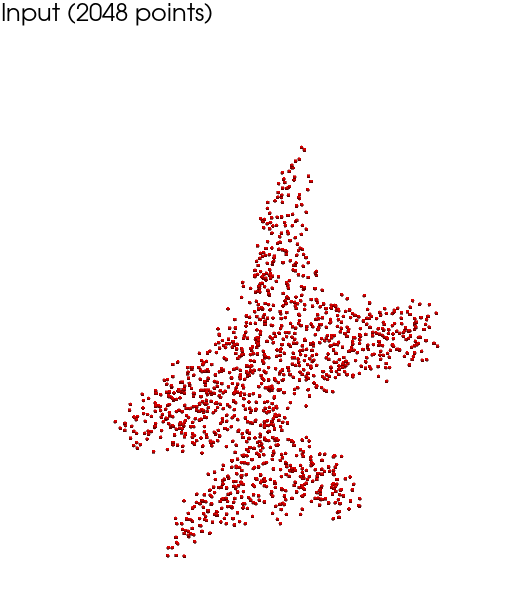
\includegraphics[width=0.6\textwidth]{figures/pointcloud/airplane/scan.png}
\caption{Projected-ShapeNet飞机样本模拟扫描位姿}
\label{fig:airplane_scan}
\end{figure}

图\ref{fig:airplane_compare}、\ref{fig:airplane_compare2}、\ref{fig:airplane_compare3}从同一视角展示了飞机样本由本算法与baseline方法的补全前后对比。左侧为输入的残缺点云（红色点云，2048个点），中间为PoinTr基线方法的补全结果（绿色点云，8192个点），右侧为本算法优化后的补全结果（蓝色点云，8192个点）。

\begin{figure}[htbp]
\centering
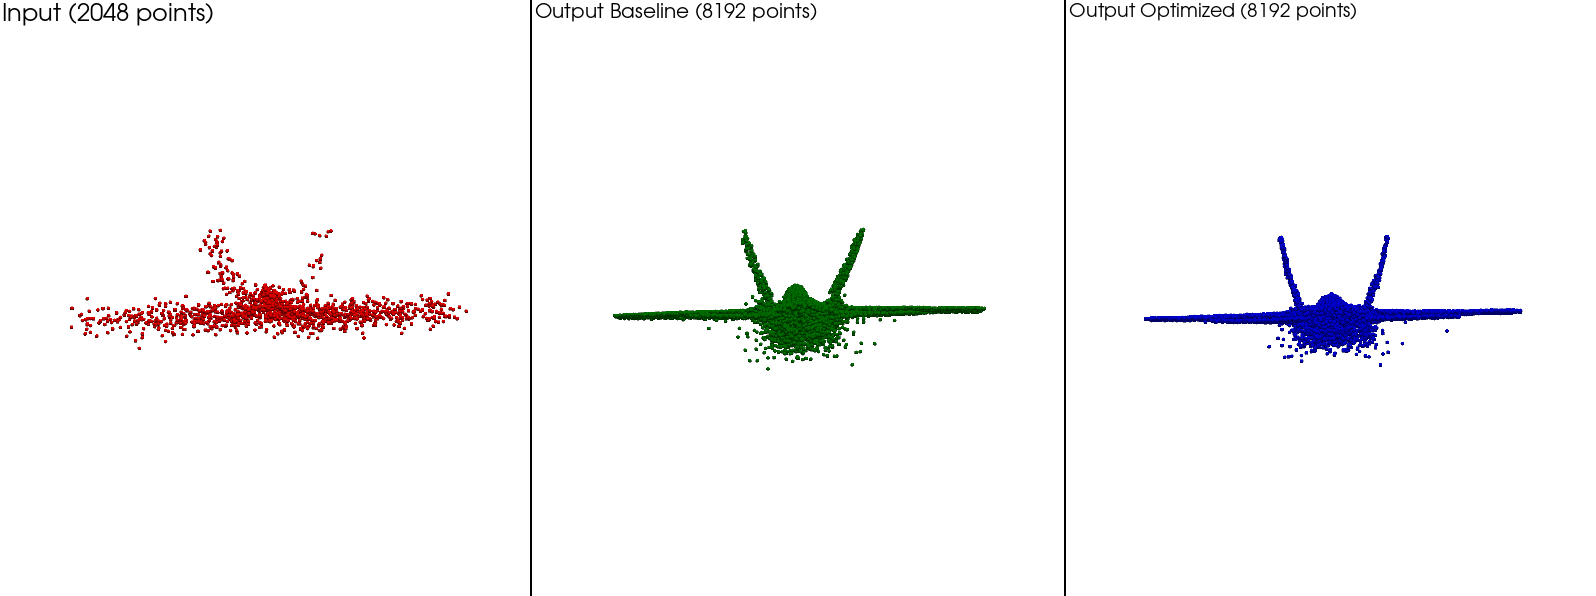
\includegraphics[width=\textwidth]{figures/pointcloud/airplane/compare-1.png}
\caption{飞机补全效果对比（视角一）}
\label{fig:airplane_compare}
\end{figure}

从图\ref{fig:airplane_compare}可以看出，在正视图视角下，PoinTr基线方法虽然能够重建出飞机的基本轮廓，但机身下方区域存在明显离群点，导致整体形状不清晰。相比之下，本算法优化后的补全结果在机身下方区域的点分布更加均匀，离群点较少，轮廓清晰，机翼与机身的过渡更加自然。

\begin{figure}[htbp]
\centering
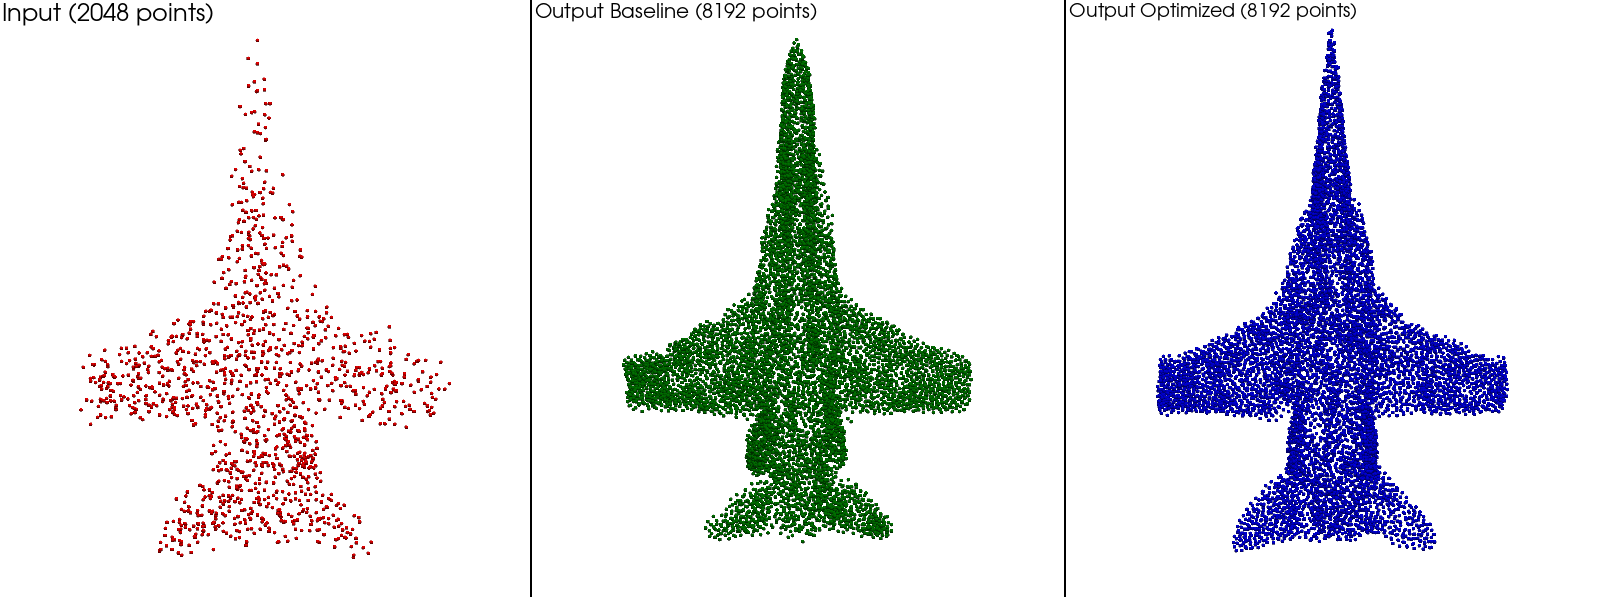
\includegraphics[width=\textwidth]{figures/pointcloud/airplane/compare-2.png}
\caption{飞机补全效果对比（视角二）}
\label{fig:airplane_compare2}
\end{figure}

图\ref{fig:airplane_compare2}从底部仰视视角展示了补全效果。在此视角下，PoinTr基线方法生成的点云在尾翼区域存在明显的原始点云缺失区域补全后局部密度不均的问题。本算法的补全结果则呈现出更加均匀的点分布，全局点密度保持一致，整体几何结构更加完整。

\begin{figure}[htbp]
\centering
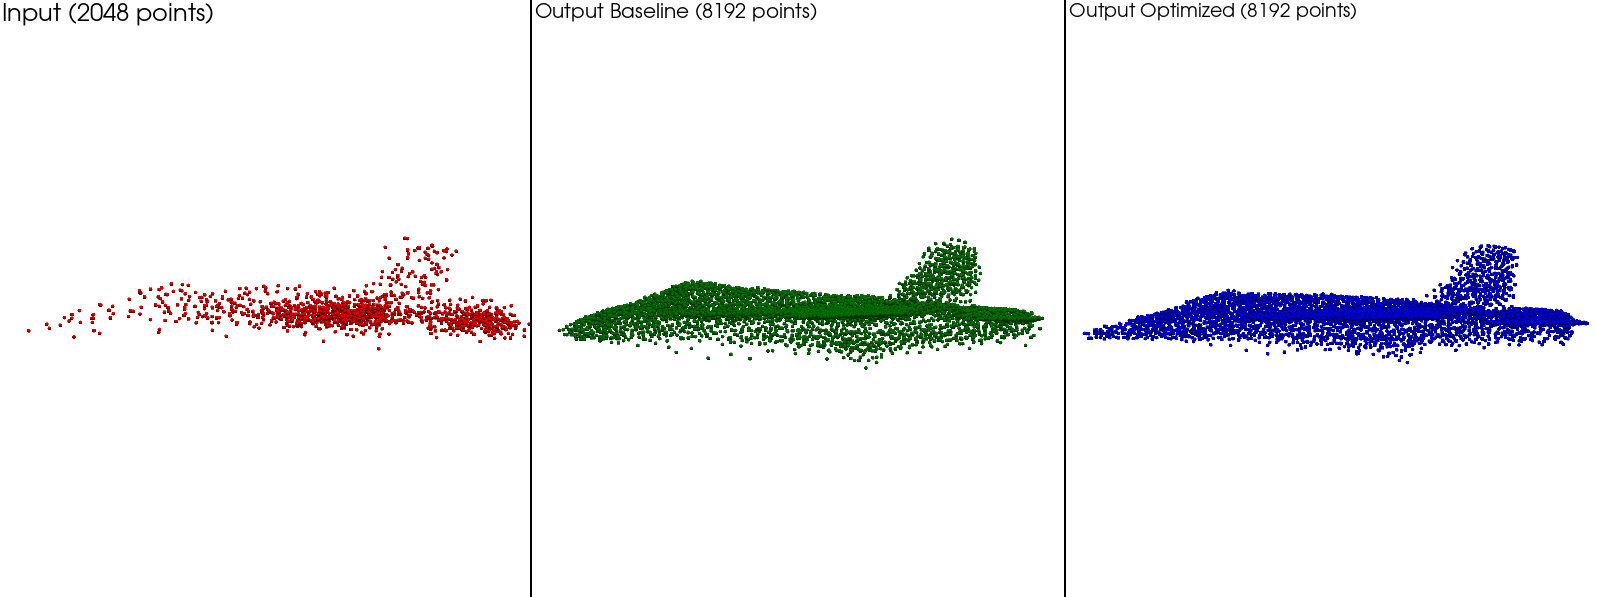
\includegraphics[width=\textwidth]{figures/pointcloud/airplane/compare-3.png}
\caption{飞机补全效果对比（视角三）}
\label{fig:airplane_compare3}
\end{figure}

图\ref{fig:airplane_compare3}从侧面视角展示了补全效果。在此视角下，PoinTr基线方法在机身腹部区域出现了严重的点云离群和密度现象。本算法通过引入DCD损失和排斥损失，有效抑制了局部点云堆积，使得机身腹部的点分布更加贴合真实表面，整体轮廓清晰，线条流畅，无明显密度不均问题。

\begin{figure}[htbp]
\centering
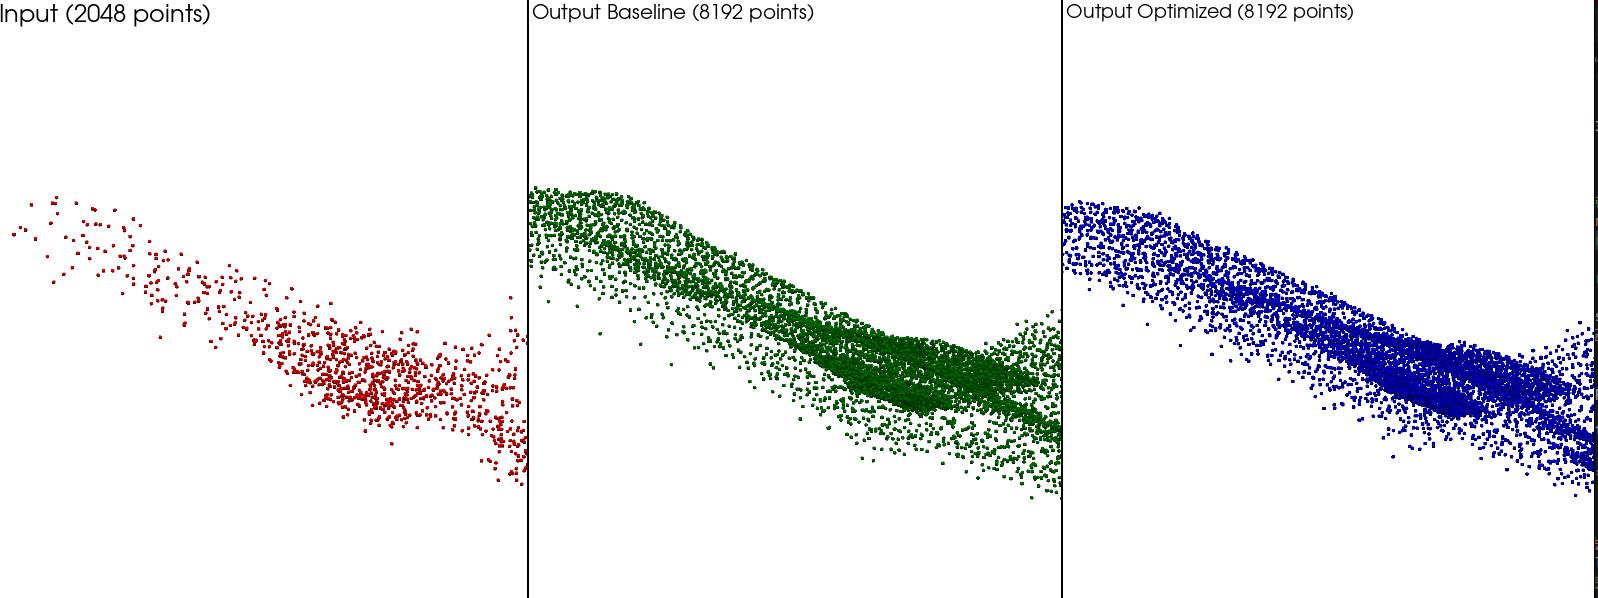
\includegraphics[width=\textwidth]{figures/pointcloud/airplane/density.png}
\caption{飞机残缺区域补全密度细节对比}
\label{fig:airplane_density}
\end{figure}

图\ref{fig:airplane_density}聚焦于飞机下防残缺区域的补全细节。从图中可以清晰地观察到，PoinTr基线方法在补全区域出现了明显的点云分层和密度不均现象，上半部分点云过度密集而需要补全的下半部分则过于洗漱。本算法的补全结果则展现出与全局密度高度一致的点分布，补全区域的点密度与原始观测区域相匹配，点云表面连续且均匀，有效验证了DCD损失和排斥损失在改善点云分布均匀性方面的作用。

(2) 吉他类别补全效果分析

图\ref{fig:guitar_scan}展示了Projected-ShapeNet数据集中吉他样本的模拟扫描位姿，本小节中Projected-ShapeNet模拟的扫描设备位于吉他上方，因此残缺点云集中在琴身区域。

\begin{figure}[htbp]
\centering
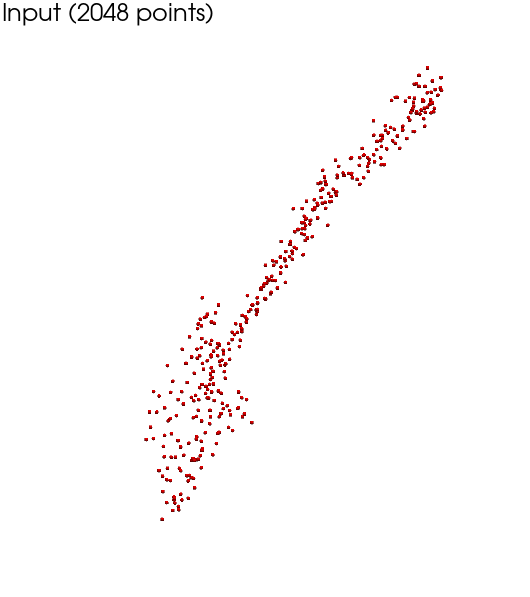
\includegraphics[width=0.6\textwidth]{figures/pointcloud/guitar/scan.png}
\caption{Projected-ShapeNet吉他样本模拟扫描位姿}
\label{fig:guitar_scan}
\end{figure}

\begin{figure}[htbp]
\centering
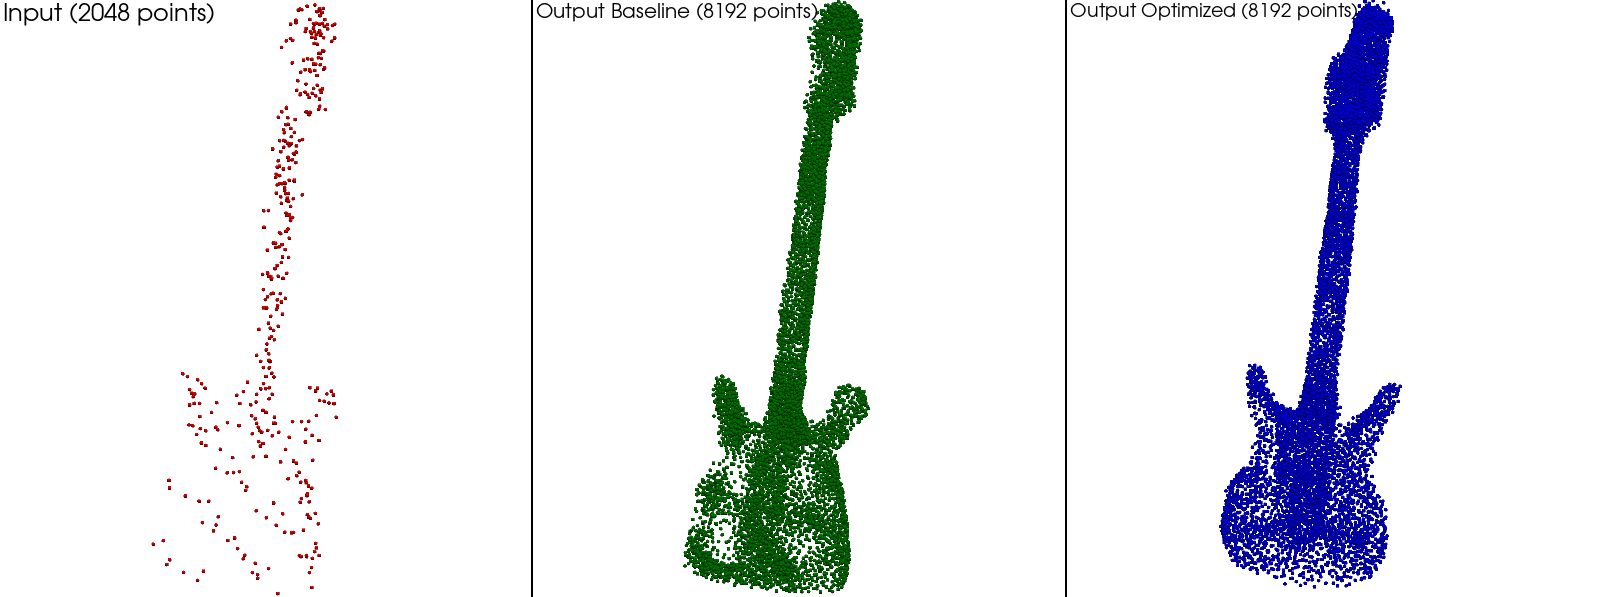
\includegraphics[width=\textwidth]{figures/pointcloud/guitar/compare-1.png}
\caption{吉他补全效果对比（视角一）}
\label{fig:guitar_compare}
\end{figure}

从图\ref{fig:guitar_compare}可以看出，在正面视角下，PoinTr基线方法虽然能够重建出吉他的基本形状，但琴身区域的点分布存在明显的不均匀现象，琴身两侧的弧形边缘处点云密度偏高，而琴身中部则相对稀疏。本算法的补全结果在琴身各区域的点密度更加均衡，琴身的弧形轮廓更加清晰，琴颈与琴身的连接处过渡更加自然。

\begin{figure}[htbp]
\centering
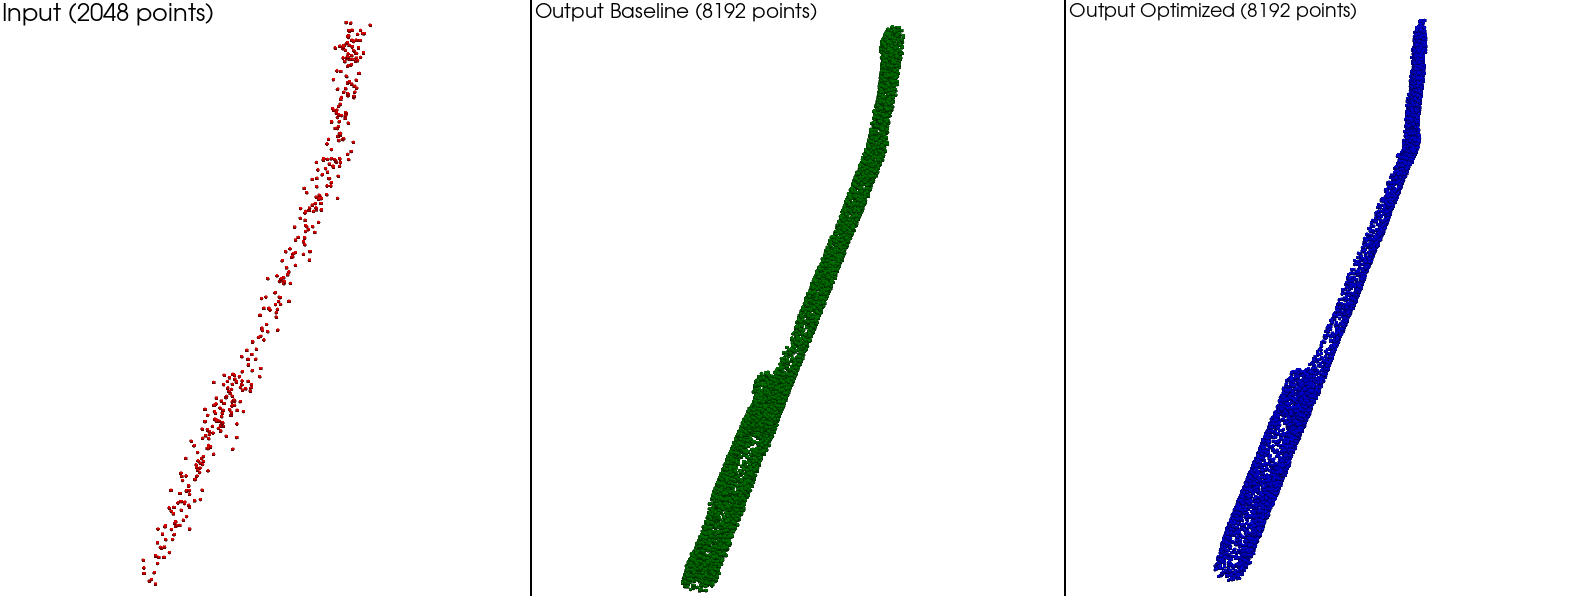
\includegraphics[width=\textwidth]{figures/pointcloud/guitar/compare-2.png}
\caption{吉他补全效果对比（视角二）}
\label{fig:guitar_compare2}
\end{figure}

图\ref{fig:guitar_compare2}从侧面视角展示了吉他琴颈的补全细节与整体轮廓。在此视角下，两个补全后的结果都没有出现明显离群点。但PoinTr基线方法生成的点云存在明显的厚度不均问题，部分区域点云过度集中导致琴颈显得过厚，而琴身与琴颈连接处过度处十分不自然，琴身也存在明显厚度不均。本算法的补全结果则呈现出均匀的琴颈厚度，轮廓清晰合理，点分布沿琴颈轴向保持一致，琴颈的几何结构更加精确。

\begin{figure}[htbp]
\centering
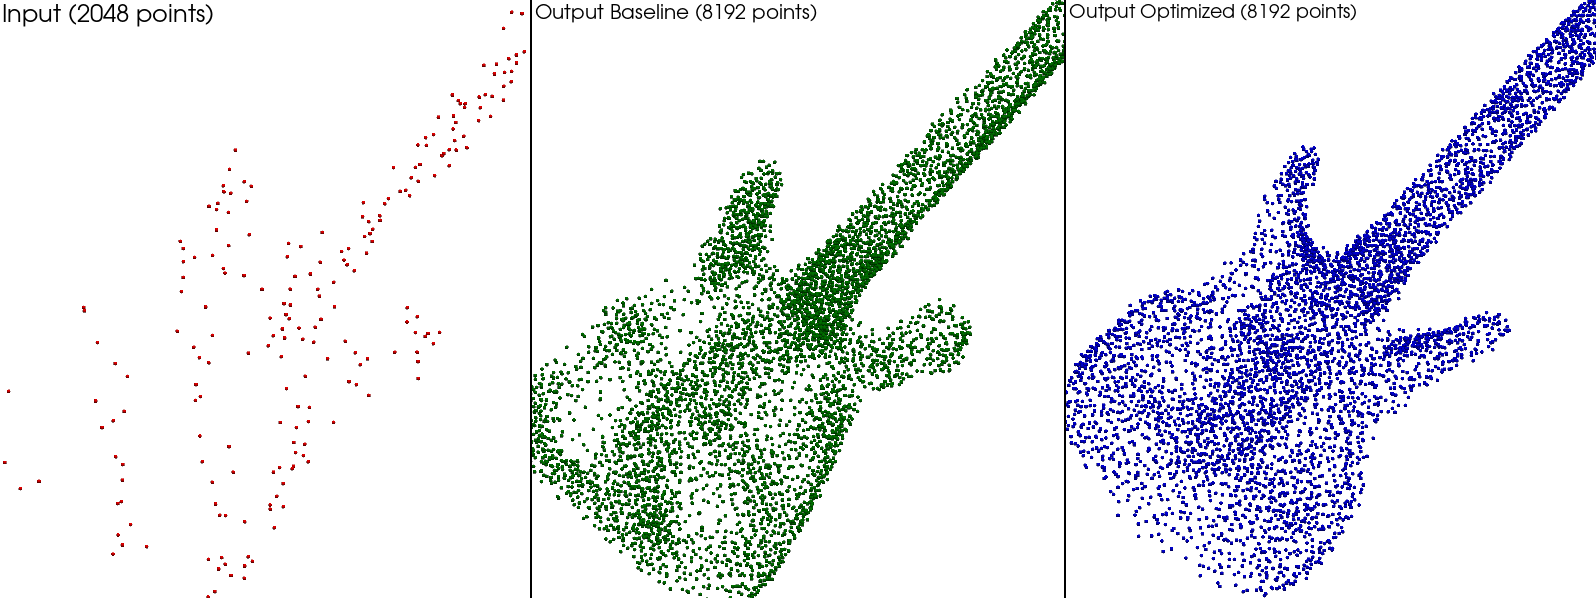
\includegraphics[width=\textwidth]{figures/pointcloud/guitar/density.png}
\caption{吉他残缺区域补全密度细节对比}
\label{fig:guitar_density}
\end{figure}

图\ref{fig:guitar_density}聚焦于吉他琴身残缺区域的补全细节。从图中可以清晰地观察到，PoinTr基线方法在琴身补全区域出现了点云密度波动现象，琴颈表面的点分布不够连续。本算法的补全结果则展现出均匀且连续的点分布，补全区域的点密度与琴身区域保持一致，琴颈表面的几何细节得到了精确还原。

(3) 可视化对比总结

综合上述可视化对比结果，本算法在点云补全效果上相较于PoinTr基线方法展现出以下优势：

（1）点云分布均匀性显著改善。通过引入DCD损失和排斥损失，本算法有效抑制了补全区域的局部点云堆积现象，使得生成点云在全局范围内保持均匀的密度分布。这一改进在飞机机身腹部、吉他琴身弧形边缘等复杂几何区域尤为明显。

（2）总体补全精度提升。本算法的补全结果在整体形状还原和局部细节精确性上均优于基线方法，补全点云与真实形状的几何偏差更小，表面连续性更好，轮廓清晰又不失细节。

（3）残缺区域补全质量提高。在结构性缺失区域，本算法能够生成与原始观测区域密度匹配的补全点云，避免了基线方法中常见的点云分层和密度波动问题，为后续的三维表面重建等下游任务提供了更高质量的输入数据。

\section{点云补全算法消融实验}

为了论证本文中优化方法的有效性，本章将使用逐步消融策略进行消融实验。与4.2.2小节相同，本章仍然采用PoinTr\cite{yu2021pointr}作为基线方法开展消融实验。

\subsection{粗粒度损失函数优化引入的影响}

PoinTr在粗粒度阶段仅使用标准CD损失进行优化，本算法在此基础上引入EMD损失，形成EMD与CD的加权组合损失。EMD通过双射匹配约束强化了骨架点云的全局拓扑对齐，而CD则保持了局部几何特征的精确性。

表\ref{tab:ablation_coarse}展示了粗粒度损失函数优化的消融实验结果。实验在ShapeNet-34数据集上进行，评价指标包括CD-L2在三种残缺程度下的表现以及F-Score@1\%。

\begin{table}[htbp]
\centering
\caption{粗粒度损失函数优化消融实验结果}
\label{tab:ablation_coarse}
\begin{tabular}{lccccc}
\toprule
\multirow{2}{*}{配置} & \multicolumn{4}{c}{CD-L2 ($\times 10^{-3}$)} & \multirow{2}{*}{F-Score@1\% ($\times 10^{-2}$)} \\
\cmidrule(lr){2-5}
& Simple & Moderate & Hard & Avg & \\
\midrule
PoinTr基线 & 0.76 & 1.05 & 1.88 & 1.23 & 42.1 \\
+ EMD损失 & 0.68 & 0.93 & 1.65 & 1.09 & 43.2 \\
\midrule
\textbf{提升幅度} & \textbf{10.5\%} & \textbf{11.4\%} & \textbf{12.2\%} & \textbf{11.4\%} & \textbf{2.6\%} \\
\bottomrule
\end{tabular}
\end{table}

从表\ref{tab:ablation_coarse}可以看出，引入EMD损失后，模型在CD-L2指标上取得了显著提升。平均CD-L2从$1.23 \times 10^{-3}$降至$1.09 \times 10^{-3}$，降幅达11.4\%。在不同残缺程度下，EMD损失的引入均带来了稳定的性能提升，其中在困难场景下的提升幅度最大（12.2\%），这表明EMD的双射匹配约束对于高缺失率情况下的全局拓扑重建具有更强的指导作用。

EMD损失的核心优势在于其对全局分布的敏感性。标准CD损失通过最近邻匹配计算预测点与真实点之间的距离，这种匹配方式允许多个预测点匹配到同一个真实点，容易导致局部点云堆积。EMD则要求建立预测点与真实点之间的一一对应关系，迫使模型在生成粗粒度点云时更加关注全局分布的均匀性。对于点云补全任务而言，粗粒度点云的全局拓扑正确性是后续细粒度优化的基础，EMD损失的引入为模型提供了更强的全局约束，使得生成的骨架点云更加接近真实形状的整体轮廓。

此外，EMD损失的引入也带来了F-Score@1\%指标的提升，从42.1\%增至43.2\%。这表明粗粒度点云质量的改善不仅体现在CD指标上，也反映在生成点云与真实点云的局部匹配精度上。高质量的粗粒度点云为后续的细粒度优化提供了更好的起点，使得模型能够在正确的全局结构基础上进行局部细节的完善。

\subsection{自适应查询生成机制影响分析}

在粗粒度损失函数优化的基础上，本实验进一步引入自适应查询生成机制。该机制包含两个关键组件：自适应查询排序和去噪任务辅助训练。自适应查询排序通过学习性重要性评估来优化查询点的选择，优先选择几何特征丰富区域的点作为查询；去噪任务辅助训练则通过在训练过程中引入额外的去噪目标来增强模型的鲁棒性和泛化能力。

表\ref{tab:ablation_query}展示了自适应查询生成机制的消融实验结果。

\begin{table}[htbp]
\centering
\caption{自适应查询生成机制消融实验结果}
\label{tab:ablation_query}
\begin{tabular}{lccccc}
\toprule
\multirow{2}{*}{配置} & \multicolumn{4}{c}{CD-L2 ($\times 10^{-3}$)} & \multirow{2}{*}{F-Score@1\% ($\times 10^{-2}$)} \\
\cmidrule(lr){2-5}
& Simple & Moderate & Hard & Avg & \\
\midrule
+ EMD损失 & 0.68 & 0.93 & 1.65 & 1.09 & 43.2 \\
+ 查询排序 & 0.61 & 0.84 & 1.48 & 0.98 & 44.1 \\
+ 去噪任务 & 0.57 & 0.78 & 1.38 & 0.91 & 44.7 \\
\midrule
\textbf{总提升幅度} & \textbf{16.2\%} & \textbf{16.1\%} & \textbf{16.4\%} & \textbf{16.5\%} & \textbf{3.5\%} \\
\bottomrule
\end{tabular}
\end{table}

从表\ref{tab:ablation_query}可以看出，自适应查询生成机制的两个组件均对模型性能产生了积极影响。引入查询排序后，平均CD-L2从$1.09 \times 10^{-3}$降至$0.98 \times 10^{-3}$，降幅达10.1\%。查询排序机制通过学习性重要性评估，使得模型能够自动识别几何特征丰富的关键区域，并将有限的查询点资源分配给最具信息量的位置。这种自适应的查询点选择策略相比于固定的FPS采样，能够更好地适应不同物体的几何复杂度分布，从而提升整体补全质量。

在查询排序的基础上进一步引入去噪任务后，平均CD-L2继续降至$0.91 \times 10^{-3}$，额外降幅为7.1\%。去噪任务的引入为模型提供了额外的监督信号，使得模型不仅需要学习如何从部分观测推断完整形状，还需要学习如何从带噪声的输入中恢复准确的几何位置。这种多任务学习策略增强了模型对输入扰动的容忍度，提升了在未见数据上的泛化性能。

自适应查询排序和去噪任务辅助训练之间存在协同效应。查询排序确保了查询点的质量，使得解码器能够基于最具信息量的查询点进行细粒度生成；去噪任务则通过额外的监督信号增强了模型对查询点特征的利用效率。两者的结合使得模型在CD-L2指标上累计提升了16.5\%，F-Score@1\%从43.2\%增至44.7\%。

\subsection{细粒度损失函数优化引入的影响}

在前两项优化的基础上，本实验最后引入细粒度损失函数优化。PoinTr在细粒度阶段仅使用标准CD损失进行优化，本算法在此基础上引入DCD损失和排斥损失，形成多损失协同优化的策略。DCD通过密度感知权重防止多个预测点匹配到同一个真实点，排斥损失则通过惩罚过近的点对来促使点云均匀分布。

表\ref{tab:ablation_fine}展示了细粒度损失函数优化的消融实验结果。

\begin{table}[htbp]
\centering
\caption{细粒度损失函数优化消融实验结果}
\label{tab:ablation_fine}
\begin{tabular}{lccccc}
\toprule
\multirow{2}{*}{配置} & \multicolumn{4}{c}{CD-L2 ($\times 10^{-3}$)} & \multirow{2}{*}{F-Score@1\% ($\times 10^{-2}$)} \\
\cmidrule(lr){2-5}
& Simple & Moderate & Hard & Avg & \\
\midrule
+ 自适应查询生成机制 & 0.57 & 0.78 & 1.38 & 0.91 & 44.7 \\
+ DCD损失\&排斥损失 & 0.51 & 0.67 & 1.19 & 0.79 & 45.5 \\
\midrule
\textbf{总提升幅度} & \textbf{10.5\%} & \textbf{14.1\%} & \textbf{13.8\%} & \textbf{13.2\%} & \textbf{1.8\%} \\
\bottomrule
\end{tabular}
\end{table}

从表\ref{tab:ablation_fine}可以看出，细粒度损失函数优化的两个组件均对模型性能产生了显著影响。引入DCD损失与排斥损失后，平均CD-L2降至$0.79 \times 10^{-3}$，降幅达13.2\%。DCD通过密度感知权重机制，有效识别和惩罚那些导致局部点云堆积的预测结果，促使生成的点云更加均匀地分布在真实点云的表面。与标准CD相比，DCD对局部密度变化更加敏感，能够更好地捕捉细粒度点云的分布质量。而排斥损失的作用机制类似于物理系统中的排斥力，当两个点之间的距离小于某个阈值时，会产生一个排斥力将它们推开，从而避免点的过度聚集。排斥损失与DCD损失的协同作用使得细粒度点云在全局结构正确的基础上，具备了更加均匀和自然的点分布特性。两者综合极大提升了模型的密度感知能力，针对原始点云残缺区域的补全密度失衡的痛点问题进行了针对性解决。

综合三项优化措施，本算法相较于PoinTr基线在CD-L2指标上累计提升了35.8\%（从$1.23 \times 10^{-3}$降至$0.79 \times 10^{-3}$），F-Score@1\%提升了8.1\%（从42.1\%增至45.5\%）。表\ref{tab:ablation_summary}汇总了完整的消融实验结果。

\begin{table}[htbp]
\centering
\caption{完整消融实验结果汇总}
\label{tab:ablation_summary}
\begin{tabular}{lccccc}
\toprule
\multirow{2}{*}{配置} & \multicolumn{4}{c}{CD-L2 ($\times 10^{-3}$)} & \multirow{2}{*}{F-Score@1\% ($\times 10^{-2}$)} \\
\cmidrule(lr){2-5}
& Simple & Moderate & Hard & Avg & \\
\midrule
PoinTr基线 & 0.76 & 1.05 & 1.88 & 1.23 & 42.1 \\
+ 粗粒度损失优化 & 0.68 & 0.93 & 1.65 & 1.09 & 43.2 \\
+ 自适应查询生成机制 & 0.57 & 0.78 & 1.38 & 0.91 & 44.7 \\
+ 细粒度损失优化 & 0.51 & 0.67 & 1.19 & 0.79 & 45.5 \\
\midrule
\textbf{总提升幅度} & \textbf{32.9\%} & \textbf{36.2\%} & \textbf{36.7\%} & \textbf{35.8\%} & \textbf{8.1\%} \\
\bottomrule
\end{tabular}
\end{table}

从表\ref{tab:ablation_summary}可以看出，三项优化措施基本独立且互补，共同推动了模型性能的提升。粗粒度损失优化主要改善了全局拓扑结构的正确性，为后续优化奠定了良好的基础；自适应查询生成机制提升了查询点的质量和模型对查询点特征的利用效率；细粒度损失优化则进一步改善了生成点云的分布均匀性和局部细节质量。三者的协同作用使得本算法在ShapeNet-34数据集上取得了显著优于PoinTr基线的补全性能。

\section{三维表面重建算法结果展示与分析}

点云补全作为三维视觉领域的基础任务，其最终目的是为下游应用提供高质量的三维几何数据。为了验证本算法优化后的补全点云在实际应用中的价值，本节将补全结果输入第三章所述的泊松表面重建流程，生成三角网格模型，并从可视化角度分析补全算法优化对三维表面重建效果的积极影响。

(1) 飞机类别重建结果分析

图\ref{fig:reconstruct_airplane_front}和图\ref{fig:reconstruct_airplane_back}分别展示了基于PoinTr基线补全点云和本算法优化补全点云重建的飞机网格模型的正面和背面视图。

\begin{figure}[htbp]
\centering
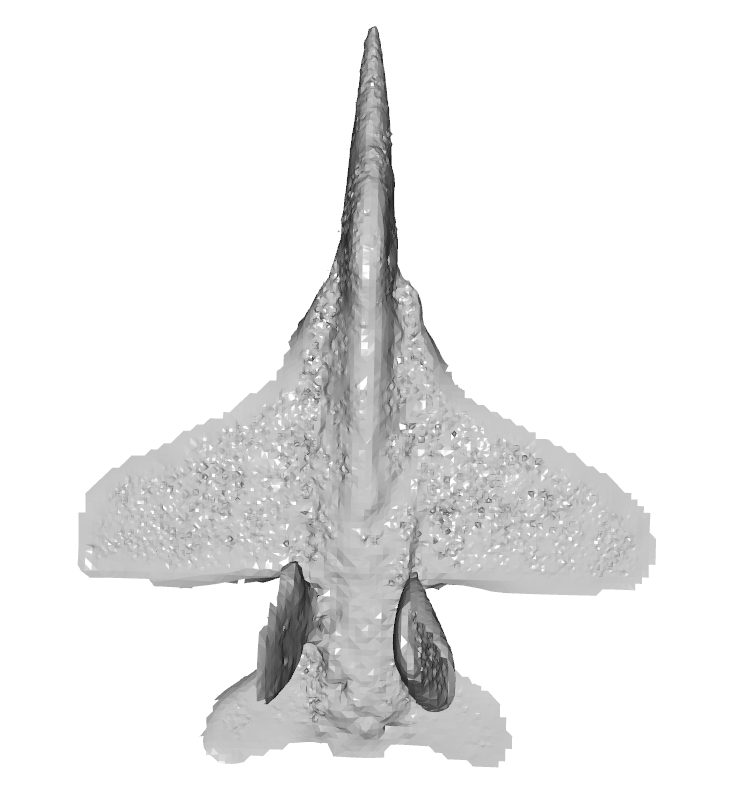
\includegraphics[width=0.45\textwidth]{figures/reconstruct/airplane/baseline-front.png}
\hfill
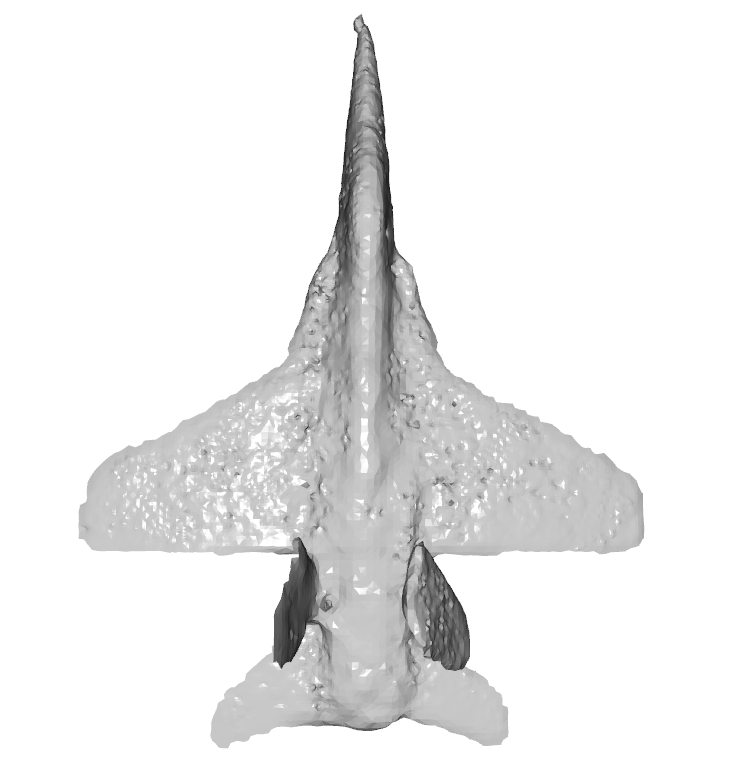
\includegraphics[width=0.45\textwidth]{figures/reconstruct/airplane/optimized-front.png}
\caption{飞机网格重建结果俯视视图对比（左：PoinTr基线，右：本算法优化）}
\label{fig:reconstruct_airplane_front}
\end{figure}

\begin{figure}[htbp]
\centering
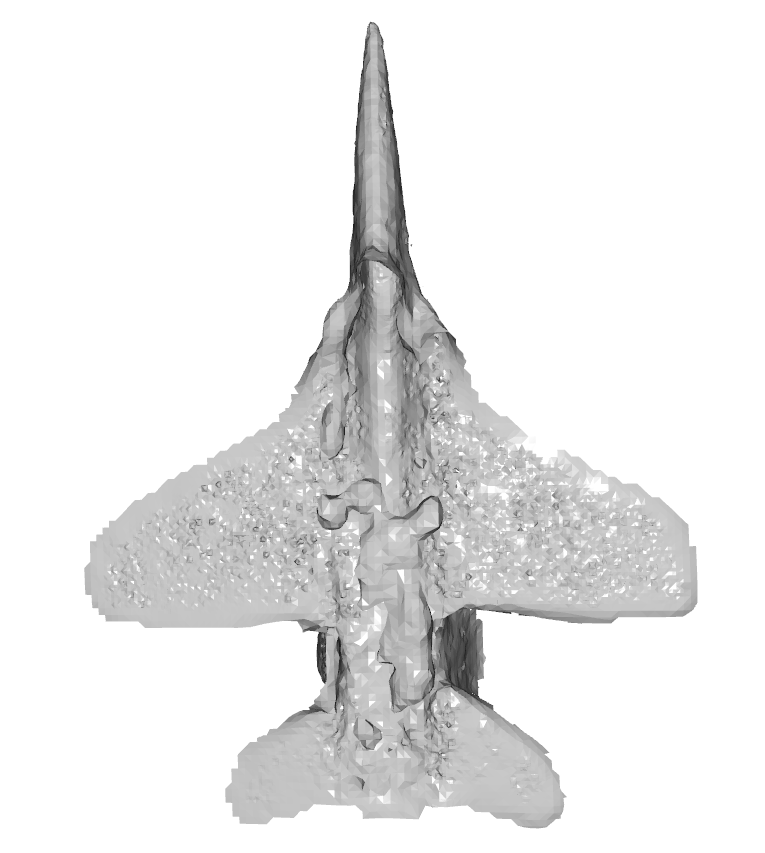
\includegraphics[width=0.45\textwidth]{figures/reconstruct/airplane/baseline-back.png}
\hfill
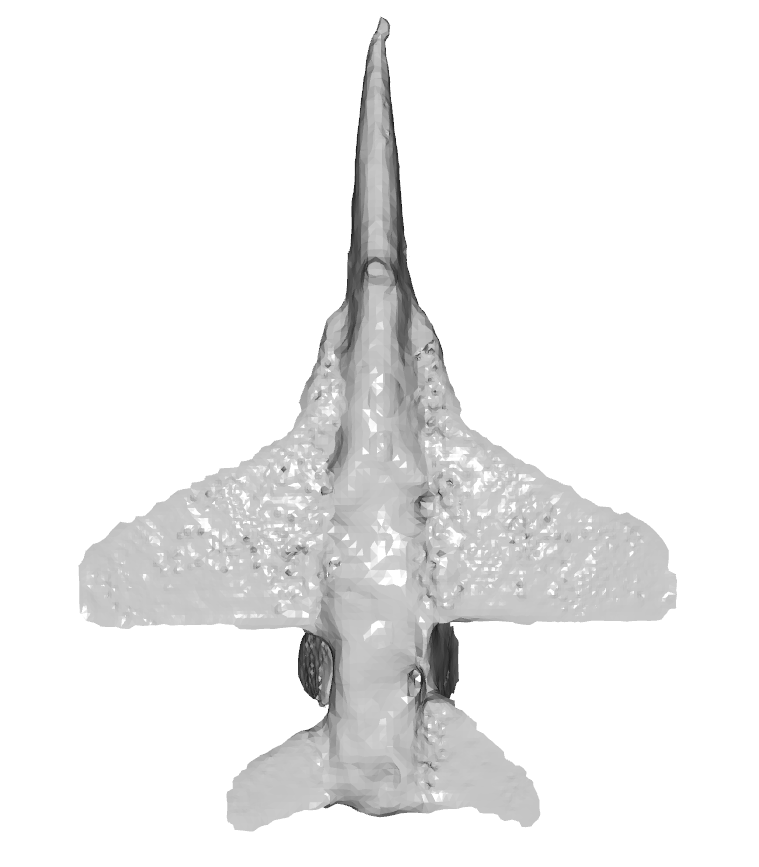
\includegraphics[width=0.45\textwidth]{figures/reconstruct/airplane/optimized-back.png}
\caption{飞机网格重建结果仰视视图对比（左：PoinTr基线，右：本算法优化）}
\label{fig:reconstruct_airplane_back}
\end{figure}

从正面视图对比可以看出，基于PoinTr基线补全点云重建的网格模型在机身背部区域存在明显的表面粗糙和局部凹陷现象。这是由于基线方法在补全过程中产生的点云堆积和密度不均导致泊松重建算法在该区域生成了不规则的三角面片，进而形成网格表面的凹凸不平。相比之下，基于本算法优化补全点云重建的网格模型在机身腹部区域呈现出光滑连续的表面，原有的凹陷和粗糙区域得到了有效修复。这一改善直接归因于本算法引入的损失函数优化对点云分布均匀性的改善，使得补全区域的点密度与全局保持一致，为泊松重建提供了更加可靠的输入数据。

从背面视图对比可以进一步观察到，基线方法重建的网格在机翼与机身连接处存在明显的边界模糊和表面断裂现象，机身腹部更是几乎完全被空洞占据。这是由于基线补全点云在该区域的轮廓不够清晰，点分布存在局部稀疏和空洞，导致法线估计不准确，进而影响泊松重建的质量。本算法优化后的补全点云在机翼与机身连接处具有更加清晰的轮廓和均匀的点分布，使得重建网格在该区域的表面连续性显著提升，机翼的几何结构得到了更加精确的还原。

(2) 吉他类别重建结果分析

图\ref{fig:reconstruct_guitar_front}和图\ref{fig:reconstruct_guitar_back}分别展示了基于PoinTr基线补全点云和本算法优化补全点云重建的吉他网格模型的正面和背面视图。

\begin{figure}[htbp]
\centering
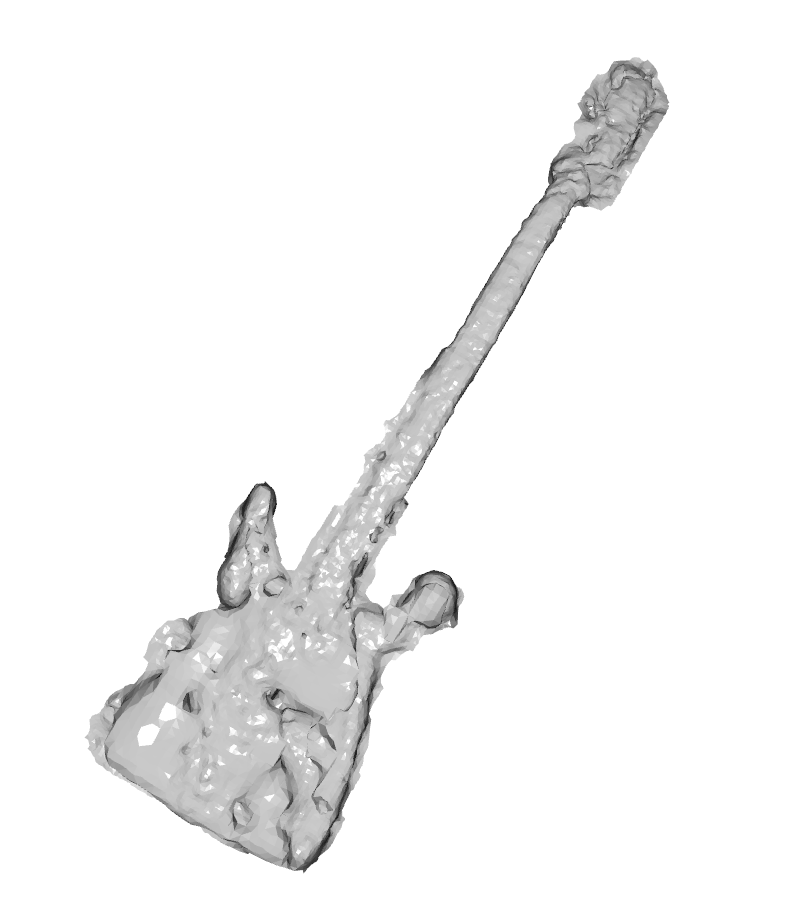
\includegraphics[width=0.45\textwidth]{figures/reconstruct/guitar/baseline-front.png}
\hfill
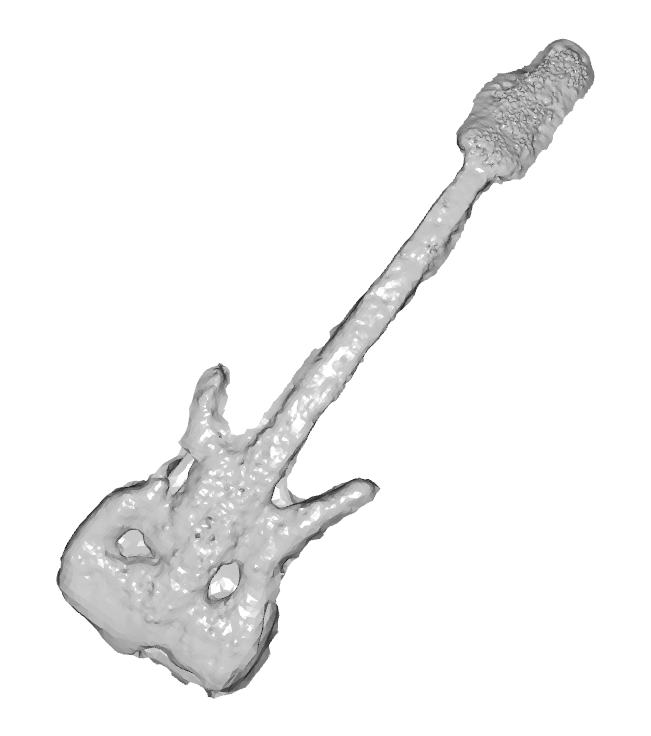
\includegraphics[width=0.45\textwidth]{figures/reconstruct/guitar/optimized-front.png}
\caption{吉他网格重建结果正面视图对比（左：PoinTr基线，右：本算法优化）}
\label{fig:reconstruct_guitar_front}
\end{figure}

\begin{figure}[htbp]
\centering
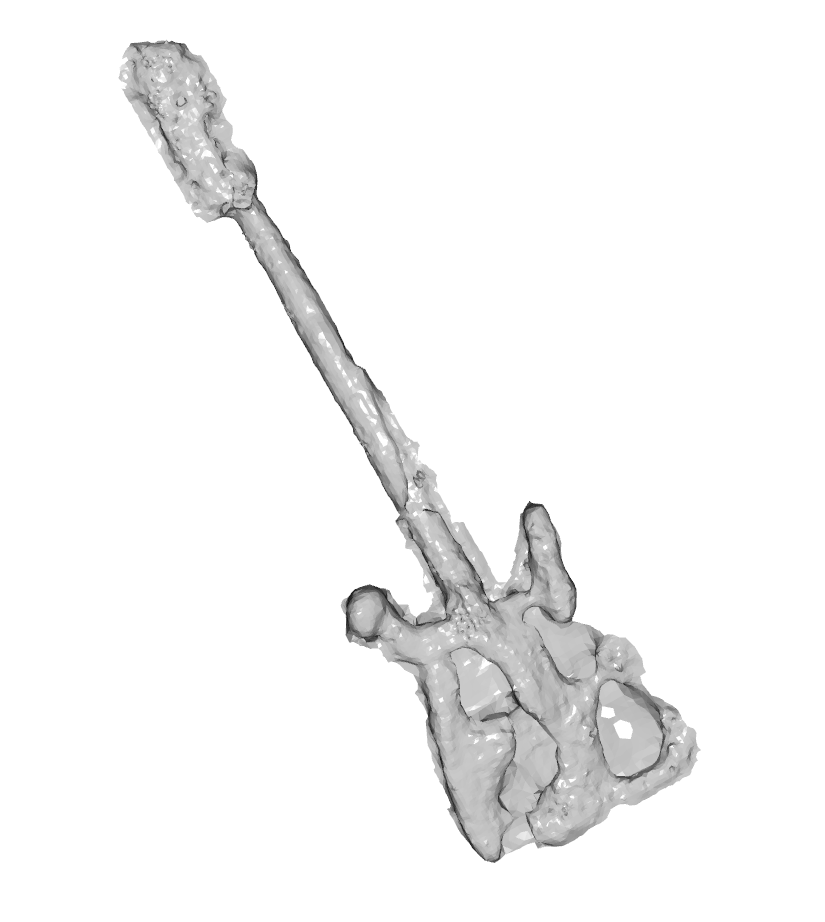
\includegraphics[width=0.45\textwidth]{figures/reconstruct/guitar/baseline-back.png}
\hfill
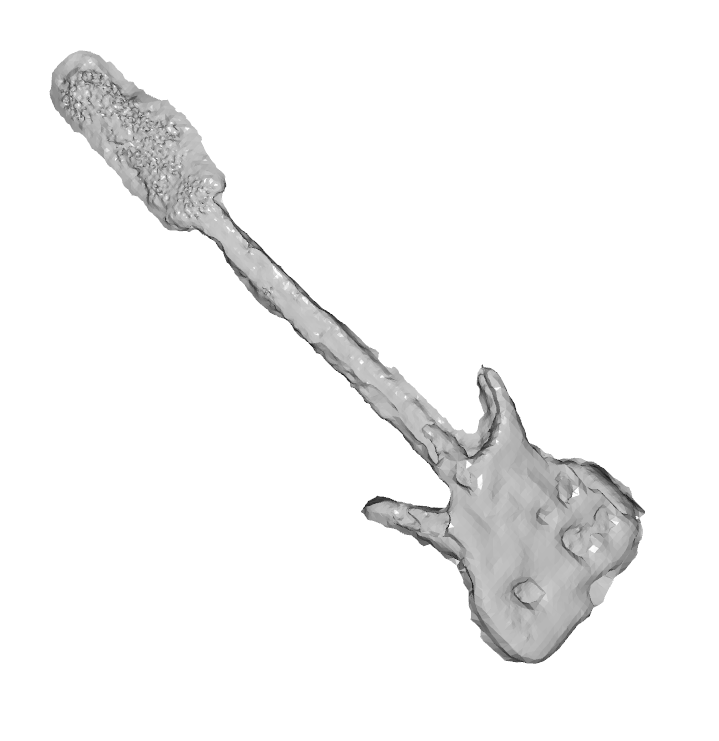
\includegraphics[width=0.45\textwidth]{figures/reconstruct/guitar/optimized-back.png}
\caption{吉他网格重建结果背面视图对比（左：PoinTr基线，右：本算法优化）}
\label{fig:reconstruct_guitar_back}
\end{figure}

从正面视图对比可以看出，基于PoinTr基线补全点云重建的吉他网格模型在琴身弧形边缘处存在明显的表面锯齿和局部变形。这是由于基线方法在补全琴身弧形区域时产生的点云密度波动，导致泊松重建算法在该区域生成了不规则的三角面片分布。相比之下，基于本算法优化补全点云重建的吉他网格模型在琴身各区域的表面更加光滑，弧形边缘的轮廓更加清晰，琴身的整体几何形状得到了更加精确的还原。

从背面视图对比可以观察到，基线方法重建的网格在琴颈区域存在明显的表面不连续和局部空洞现象。这是由于基线补全点云在琴颈区域的点分布不够均匀，部分区域点云过于密集而另一些区域则出现稀疏，导致法线估计和泊松重建在该区域的质量下降。本算法优化后的补全点云在琴颈区域呈现出均匀且连续的点分布，使得重建网格在该区域的表面质量显著提升，琴颈的几何结构得到了更加精确的还原。

(3) 重建结果综合分析

综合上述重建结果对比，本算法优化后的补全点云为三维表面重建带来了以下积极影响：

（1）轮廓清晰度提升。本算法通过自适应查询生成机制和混合损失函数优化，使得补全点云在物体边缘和结构转折处的轮廓更加清晰。清晰的点云轮廓为法线估计提供了更加准确的局部几何信息，进而提升了泊松重建的表面质量。

（2）点云分布均匀性改善。本算法引入的损失函数优化有效抑制了补全区域的局部点云堆积和空洞现象，使得生成点云在全局范围内保持均匀的密度分布。均匀的点分布为泊松重建提供了更加可靠的输入数据，减少了重建过程中因点密度波动导致的表面粗糙和局部变形。

（3）整体精度提升。本算法优化后的补全点云在整体形状还原和局部细节精确性上均优于基线方法，使得重建网格模型在几何精度和表面质量上均得到了显著提升。这一改善在飞机机身腹部、吉他琴身弧形边缘等复杂几何区域尤为明显。

上述结果表明，点云补全算法的优化不仅体现在补全点云本身的定量指标提升上，更能够直接转化为下游三维表面重建任务的质量改善。本算法通过系统性的损失函数优化和查询生成机制改进，有效解决了补全区域点云密度失衡的核心问题，为三维视觉领域的实际应用提供了更加可靠的技术支撑。

\section{本章小结}

本章通过系统的实验验证了本文基于Transformer的点云补全算法的卓越性能。在ShapeNet-34数据集上的对比实验表明，本算法在CD-L2和F-Score@1\%指标上均取得了具有竞争力的结果，优于PoinTr、SnowflakeNet等经典方法。在Projected-ShapeNet数据集上的可视化对比进一步验证了本算法在点云分布均匀性和整体补全精度上的优势。消融实验结果表明，粗粒度损失优化、自适应查询生成机制和细粒度损失优化三项措施累计使CD-L2指标降低35.8\%，F-Score@1\%提升8.1\%，各项优化措施独立且互补，共同推动了模型性能的提升。三维表面重建结果展示表明，本算法优化后的补全点云能够有效改善下游重建任务的质量，在轮廓清晰度、点云分布均匀性和整体精度方面均带来积极影响，为点云补全算法的实际应用提供了有力支撑。